\section*{Problem 1}
The code listing for problem 1 is Listing~\ref{list:p1}. The \texttt{MEM\_LOC} macro was redefined for the different sizes we required (\texttt{MEM\_LOC\_CHAR} for 1 byte, \texttt{MEM\_LOC\_SHORT} for 2 bytes, and \texttt{MEM\_LOC\_INT} for 4 bytes). The required addresses were defined in the macros \texttt{LOC1}-\texttt{LOC4}, using the new macros created for \texttt{MEM\_LOC}. These macros are used in the function \texttt{problem1} to write the required values to the memory addresses.

The memory and expression panels for problem 1 are shown in Figure~\ref{fig:p1}. The endianness was set to big, the cell size to 1 byte, and the radix to hex.

\begin{lstlisting}[language=c,caption=Problem 1, label=list:p1]
/* Definitions */
#define MEM_LOC_CHAR(x)             *((char*)x)
#define MEM_LOC_SHORT(x)            *((short*)x)
#define MEM_LOC_INT(x)              *((int*)x)
#define LOC1                        MEM_LOC_CHAR(0x20001000)
#define LOC2                        MEM_LOC_INT(0x20001001)
#define LOC3                        MEM_LOC_SHORT(0x20001005)
#define LOC4                        MEM_LOC_INT(0x20001007)

/* Problem 1 Function */
void problem1() {
    LOC1 = 0xAC;
    LOC2 = 0xAABBCCDD;
    LOC3 = 0xABCD;
    LOC4 = 0xAABBCCDD;
}
\end{lstlisting}

\begin{figure}[htp]
\centering
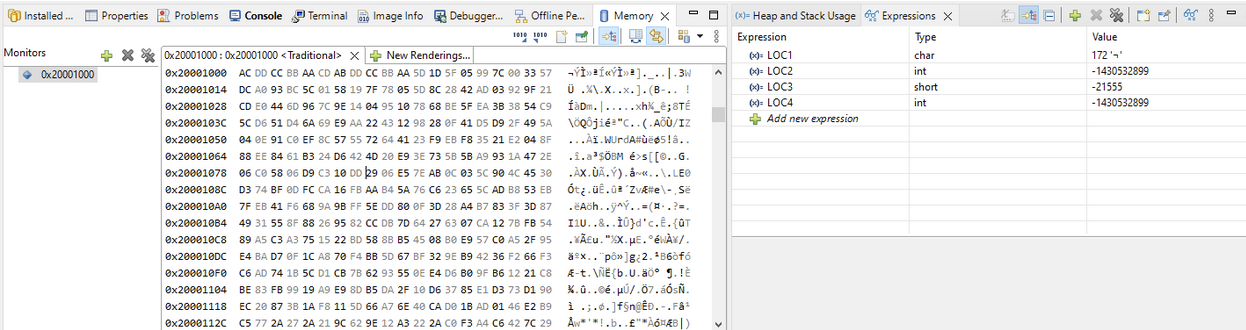
\includegraphics[width=\textwidth]{p1}
\caption[problem 1]{Memory and Expression Panels for Problem 1}\label{fig:p1}
\end{figure}